%
% http://www-d0.fnal.gov/Run2Physics/top/top_public_web_pages/top_feynman_diagrams.html
%

\chapter{Top-Quark Pair-Production Cross-Section}

A precise measurement of the Top Quark Pair-Production Cross-Section is crucial for understanding the performance of the ATLAS detector, for testing predictions of the standard model, to searching for or constraining many new physical models.
Measuring the $\ttbar$ cross-section was an early goal of the ATLAS experiment as it was accessable using a relatively small dataset and was valuable in terms of understanding the performance of the detector and searching for early signatures of new physics.
The measurement of a cross-section, which expresses the rate of a particular reaction or production mechanism independently of the amount of the beam conditions that are used to produce it,
requires a detailed understanding of process being measured, knowledge of the backgrounds that can minic that process, and measurements of the systematic uncertainties that can influence the measurement of a cross-section.
The decay topology of the $\ttbar$ system results in high-pt leptons, jets, including jets arising from $b$-quarks, and missing energy.
To perform this measurement accurately, coordination between the detector systems and performance groups used to reconstruct these physical objects was crucial.
The measurement of the $\ttbar$ cross-section was among the first major analyses to require such a large level of accuracy across a wide spectrum of the detector. % Blah

Furthermore, the production of top-quarks results in large backgrounds for a wide range of analyses.
Because the final state of $\ttbar$ can include a large number of jets, high-pt leptons, and missing energy, it enters as a background to Higgs searches, Super Symmetry searches (SUSY),
and the majority analyses searching for exotic particles.
Being able to accurately measure the rate of this background is a necessary step for nearly all searches for beyond-the-standard-model physics.

%The top-quark pair-production cross-section, which expresses the rate of a particular reaction or production mechanism independently of the amount of the beam conditions that are used to produce it.
%In particle physics, a cross-section is a way of expressing the rate of a particular reaction or production mechanism independently of the amount of the beam conditions that are used to produce it.
%to describe the rate of a specific interaction or class of interactions independently of beam conditions that are used to produce it.
The value of the top-quark pair-production cross-section in the Standard Model can be predicted using Monte-Carlo simulation techniques \cite{TOP_XSC_THEORY} \cite{Langenfeld:2009ue} \cite{THRESHOLD_EXPANSION_XSC}.
This value can be determined using ``Next to Leading Order'' techniques (NLO) and is corrected by adding the ``Next to Next to Leading Order'' soft logarithm terms (approximate NNLO).
This value is determined to be $\sigma_{\ttbar} = 165^{11}_{16}$ with an uncertainty below 10\%.
The most accurate experimental determinations of the top quark's cross section previous to the LHC's results were measured by the CDS and the D0 collaborations at the Tevatron \cite{TEVATRON_XSC_LJETS} \cite{TEVATRON_XSC_DILEP}.
These experiments determined the cross-section at a center-of-mass energy of $\sqrt{s} = 7 TeV$ to a precision of 8\% using individual channels and 6.4\% by combining measurements across multiple channels.

At ATLAS, the $\ttbar$ production cross-section can be measured using a number of final states.
In this thesis, we will describe three separate analyses that measured the $\ttbar$ cross-section using independent sets of events.
These measurements include the single-lepton, dilepton, and all-hadronic final states, which are each measured using separate and orthogonal
definitions of signal region and using differnet analysis techniques.
These three measurements are described separately in individual chapters.

A measurement combining the individual results from these separate search channels is presented in section~\ref{sec:combination}.
By using a likelihood function that describes the individual measurements and combines common parameters and sources of uncertainty,
one obtains a better measurement of the $\ttbar$ cross-section.
At the time of publication, this measurement using a statistical combination of individual analyses had the smallest uncertainties
of all measurements of the $\ttbar$ cross-section produced by either ATLAS or CMS and was comparable to the combined result from 
the Tevatron using data obtained by both the CDF and D0 experiments.


\section{Top Quark Pair-Production}

The primary means of producing top quarks at the LHC is via gluon fusion and subsequent decay into a pair of top quarks, as showin in figure ~\ref{img:TopQuarkPairProduction}.

\begin{figure}
  \begin{center}

    \subfigure[Production]{
      % TopQuarkPairProductionDiagram: http://kjende.web.cern.ch/kjende/netzwerk/images/Feynman/WplusWminusBBar.png
      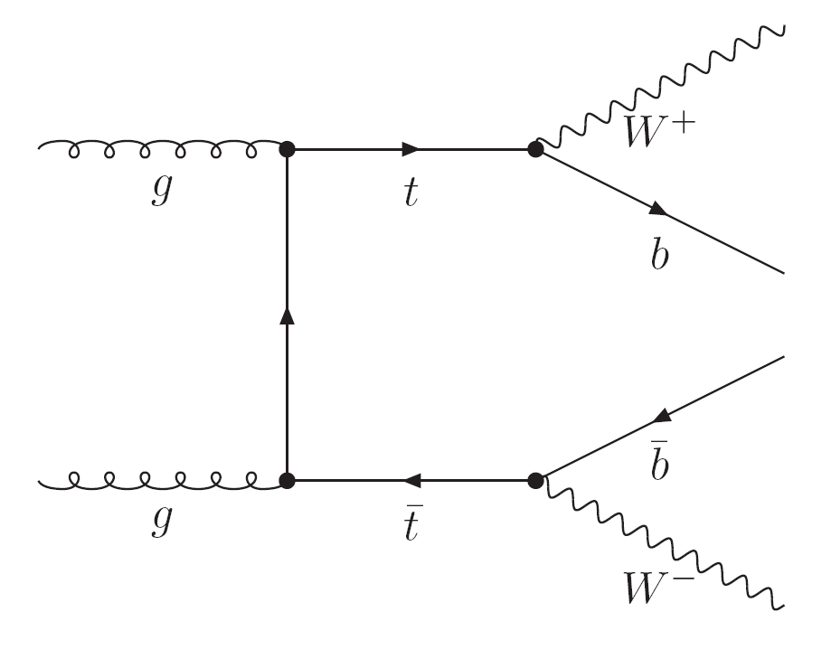
\includegraphics[width=.4\linewidth]{figures/xsection/TopQuarkPairProductionDiagram.png}
    }
    \subfigure[Decay]{
      % TopQuarkBranchingRatios: http://ej.iop.org/images/0034-4885/75/5/056201/Full/rpp347183f06_online.jpg
      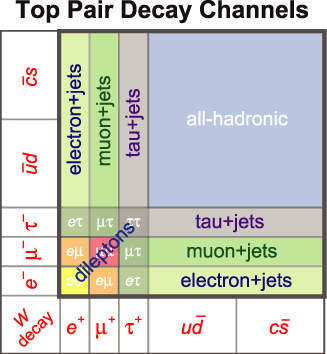
\includegraphics[width=.4\linewidth]{figures/xsection/TopQuarkBranchingRatios.jpg}
    }
  \end{center}
  \caption{A typical feynman diagram of top quark pair production at the LHC.
    Top quarks decay into W-bosons and b-quarks nearly 100\% of the time.
    The subsequent decays of the W-Bosons determine the event topology of the \ttbar event.
    Diagram showing the branching ratios of Top Quark pairs into leptons and quarks.}
  \label{img:TopQuarkPairProduction}
\end{figure}
The top quark is unstable and decays almost immediately, having a lifetime of about $5*10^{-25}$\cite{PARTICLE_DATA_GROUP}.
The top decays with a nearly 100\% branching ratio into a $b$-quark and W boson.
Thus, an intermediate state in the decay of $\ttbar$ production consists of in 2 $W$-bosons and 2 $b$-quarks.

W bosons decay either leptonically, in which they produce a lepton and a neutrino, or hadronically, in which they produce a pair of quarks.
W's decay leptonically 32.6\% of the time, which consists of decaying via $W- \rightarrow e \bar{\nu_{e}}$ 10.75\% of the time, 
via $W- \rightarrow \mu \bar{\nu_{\mu}}$ 10.57\% of the time, and via $W- \rightarrow \tau \bar{\nu_{\tau}}$ 11.25\% of the time, 
and decay into quarks the other 67.60\% of the time. \cite{PARTICLE_DATA_GROUP}
% W-Boson: http://pdg.lbl.gov/2012/listings/rpp2012-list-w-boson.pdf
However, tau leptons are themselves unstable particles that subsequently decay either leptonically (muon 17.41 or electron 17.83), or hadronically 64.76\% of the time, with about 50\% of the tau's today decays into 1 hadron and 15\% into 3 hadrons.
% Tau pdg: http://pdg.web.cern.ch/pdg/2012/listings/rpp2012-list-tau.pdf
In the discussion that follows, leptonic decays of a top quark include $t \rightarrow W \rightarrow \tau \rightarrow e$ or $t \rightarrow W \rightarrow \tau \rightarrow \mu$, and we will ignore the intermediate state $\tau$ in terms of our classification.
Hence, a pair of top quarks, which we assume always decay into a pair of W bosons, will decay into two leptons 6.5\% of the time (known as the ``dilepton'' channel), into a single lepton and a pair of quarks 34.4\% of the time (known as the ``single lepton'' channel), and entirely into quarks 45.7\% of the time (known as the ``all hadronic'' channel).
% pdg:
% Citation: J. Beringer et al. (Particle Data Group), PR D86, 010001 (2012) (URL: http://pdg.lbl.gov)

%% \begin{figure}
%%   \begin{center}
%%     % TopQuarkBranchingRatios: http://ej.iop.org/images/0034-4885/75/5/056201/Full/rpp347183f06_online.jpg
%%     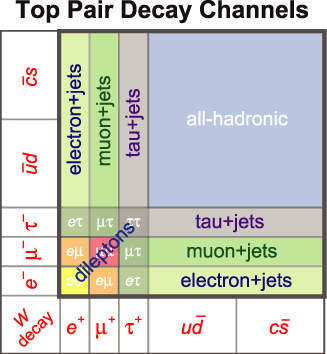
\includegraphics[width=100mm]{figures/xsection/TopQuarkBranchingRatios.jpg}
%%   \end{center}
%%   \caption{}
%%   \label{img:TopQuarkBranchingRatios}
%% \end{figure}


%% \subsection{Object Reconstruction}

%% Measurements of $\ttbar$ event require kinematicaly reconstructing and selecting a variety of physical objects, including electrons, muons, jets, b-jets, and $\MET$.

%% % Selected Electrons
%% Selected electrons are required to have a calorimeter cluster located in a pseudorapidity range of $0 < |\eta| < 4.47$, excluding the range $1.37 < |\eta| < 1.52$ (this excluded interval, known as the crack region, is a mostly un-insturmented part of the EM calorimeter).
%% To reject jets that fake electrons, the electron's energy is required to be isolated in the calorimeter.
%% Specifically, electrons with more than 3.5 GeV of energy in a cone of $\sqrt{(\Delta \eta)^2 + (\Delta \phi)^2}$, excluding the energy of the electron itself, are rejected.
%% Electrons must pass a variety of cuts related to the shape of its shower and the quality of its corresponding track that are collectively referred to as ``tight'' EM identification cuts.
%% Finally, Electrons must have a minimum energy of $E_{T} > 20$ GeV, where $E_{T}$ referrs to the transverse energy of the electron's electromagnetic cluster.

%% %% The selection of l + jets tt ̄ events makes use of reconstructed electrons, muons and jets, and the transverse momentum imbalance referred to as missing transverse energy Emiss.
%% %% T Electron candidates are reconstructed from the energy depositions in the electromagnetic calorimeter
%% %% and are required to have a well-measured track associated with the electromagnetic cluster. The latter is required to have |ηcluster| < 2.47 excluding 1.37 < |ηcluster| < 1.52 corresponding to the transition region between barrel and endcap calorimeters. To ensure that electrons are isolated from the jet activity, as expected for prompt electrons from W boson decay, the energy in a cone of ∆R ≡ 􏰮∆η2 + ∆φ2 = 0.2, centered around the electron, excluding the energy associated with the electron itself, is required to be < 3.5 GeV. This defines the tight electron candidates used for the final analysis. Loose electron candidates employed for the estimation of the QCD multijet background, as described in Section 4, have to fulfill less stringent requirements and the isolation cut is increased to < 6 GeV energy deposition in ∆R = 0.2.

%% % Selected Muons
%% Selected Muons must be ``combined'', meaning they must use tracks from both the muon spectrometer and the inner detector.
%% Only muons within $|\eta| < 2.5$ are considered, and muons within $\Delta R <= 0.4$ of a selected jet are rejected.
%% Two isolation requirements are imposed on selected muons.
%% They must be isolated in the calorimeter, meaning the energy deposited in the calorimeter within $\Delta R = 0.3$ must be $<$ 4 GeV, and their tracks must be isolated, meaning the sum of the transverse momenta of tracks in a code of $\Delta R = 0.3$ surronding the muon's track must be $<$ 4 GeV.

%% %% Muon candidates are reconstructed by searching for track segments in the different layers of the muon spectrometer. These segments are then combined starting from the outermost layer, and matched with the inner detector tracks. The final parameters of muon candidates are obtained from the combined fit using information from both detector systems. Only muons within |η| < 2.5 are included in this measurement. Like electrons, muons are required to be isolated, i.e. (i) be separated from the closest jet by ∆R(μ, jet) > 0.4; (ii) have calorimeter isolation < 4 GeV and (iii) have track isolation < 4 GeV. Track isolation is defined as the sum of track transverse momenta in a cone ∆R ≡ 􏰮∆η2 + ∆φ2 = 0.3, excluding the pT of the muon track, while calorimeter isolation is defined as energy deposition in the calorimeter within a cone of ∆R = 0.3, excluding the energy deposition directly along the muon track. Muons passing all requirements are used in the analysis sample selection and are referred to as tight, while muons with a looser isolation are used for the QCD multijet background estimate described in Section 4. In this case, all requirements except the cuts on calorimeter and track isolation have to be fulfilled and the muons are referred to as loose.

%% % Selected Jets
%% In this analysis, Jets are constructed using the anti-kt algorithm with a distance parameter of $R=0.4$.
%% These jets are built out of ``topoligical clusters'', which themselves are collections of neighboring cells that each have an energy above some threshold, where the energy has been calibrated to the scale of electromagnetic showers (known as ``Electromagnetic Scale'').
%% Once the jets are built, their energies are then recalibrated to the scale of hadronic particles (known as the ``Hadronic scale'')~\cite{JES_SCALE_2010}.
%% Since jets are built out of calorimeter deposits, essentially all electrons will also be reconstructed as jets.
%% Therefore, these objects must be removed from the collection of selected jets by-hand.
%% In this analysis, any jet that overlaps with a selected electron within $\Delta R < 0.2$ is removed.

%% %% Jets are reconstructed using the anti-kt algorithm with distance parameter R = 0.4 [9] which sets the relative distance at which jets are resolved from each other. As input, the algorithm uses topological clusters that group together neighboring calorimeter cells with energy deposits above certain thresholds. Their energy accounts correctly for the energy deposited in the calorimeter by electromagnetic showers. Additional correction factors dependent on jet η and pT are applied to the reconstructed jets to correct their energy to the hadronic scale. The jet energy scale (JES) is established using corrections derived from collision and test beam data and calibration constants obtained from MC simulation [10]. Since reconstructed electrons might also be reconstructed as jets in the calorimeter, any jet overlapping with a %% 2 %% tight electron within a cone of ∆R < 0.2 is removed from the list of jets.

%% %% MET
%% Finally, once all objects have been selected, the $\MET$ is defined as the vector sum of the calorimeter energy deposits of selected objects or the combined energy for muons (including additional corrections for energy deposited in the calorimeter).
%% The energy associated with each object is calibrated to the scale of that object, and all remaining energy deposits are added to the $\MET$ vector, but at electromagnetic scale.

%% %% The analysis reconstructs the missing transverse energy from the vector sum of energy depositions
%% %% in the calorimeter in the transverse plane associated to the objects used in the analysis. The same recon-
%% %% struction and identification algorithms as for the analysis objects are used to identify electrons and jets.
%% %% The corresponding topological clusters in the calorimeters are then included in the calculation of Emiss at T
%% %% the energy scale of the associated object. The muon momenta are calculated using the information from both the inner detector and the muon spectrometer system and corrected for additional energy deposi- tion in the calorimeter. Remaining energy depositions not associated to any object are included at the electromagnetic energy scale.

%% %% END
